% --------------------------------------------------------------
% This is all preamble stuff that you don't have to worry about.
% Head down to where it says "Start here"
% --------------------------------------------------------------
 
\documentclass[12pt]{article}

\usepackage{courier}
\usepackage{color}
\usepackage{listings}
\usepackage[square,numbers]{natbib}
\usepackage{tabls}
\usepackage{graphicx}
\usepackage{subcaption}
\usepackage{pdfpages}
\usepackage{mathtools}

\definecolor{dkgreen}{rgb}{0,0.6,0}
\definecolor{gray}{rgb}{0.5,0.5,0.5}




\lstset{language=python,
   basicstyle=\ttfamily,
   keywordstyle=\color{blue},
   commentstyle=\color{dkgreen},
   stringstyle=\color{red},
   numbers=left,
   numberstyle=\tiny\color{gray},
   stepnumber=1,
   numbersep=10pt,
   backgroundcolor=\color{white},
   tabsize=4,
   showspaces=false,
   showstringspaces=false}
 
\usepackage[margin=1in]{geometry} 
\usepackage{amsmath,amsthm,amssymb}
\usepackage{verbatim}
\usepackage{algpseudocode,algorithm}
\usepackage{setspace}

\newcommand{\ihat}{\ensuremath{\hat{\textbf{\i}}}}
\newcommand{\jhat}{\ensuremath{\hat{\textbf{\j}}}}
\newcommand{\lline}{\noindent\makebox[\linewidth]{\rule{\textwidth}{0.4pt}}}
\newcommand{\N}{\mathbb{N}}
\newcommand{\Z}{\mathbb{Z}}
\newcommand{\deriv}[2]{\frac{\mathrm{d} #1}{\mathrm{d} #2}}
\newcommand{\pderiv}[2]{\frac{\partial #1}{\partial #2}}
\newcommand{\bx}{\mathbf{X}}
\newcommand{\ba}{\mathbf{A}}
\renewcommand{\d}{\mathrm{d}}
\newcommand{\A}{\frac{(1-\alpha)}{2(1+\alpha)}}
\newcommand{\upl}{u_{\text{plane}}}
\newcommand{\upt}{u_{\text{point}}}
\newcommand{\D}{\Delta}
\newcommand{\ra}{\rightarrow}
\renewcommand{\SS}{\State}
 
\newenvironment{theorem}[2][Theorem]{\begin{trivlist}
\item[\hskip \labelsep {\bfseries #1}\hskip \labelsep {\bfseries #2.}]}{\end{trivlist}}
\newenvironment{lemma}[2][Lemma]{\begin{trivlist}
\item[\hskip \labelsep {\bfseries #1}\hskip \labelsep {\bfseries #2.}]}{\end{trivlist}}
\newenvironment{exercise}[2][Exercise]{\begin{trivlist}
\item[\hskip \labelsep {\bfseries #1}\hskip \labelsep {\bfseries #2.}]}{\end{trivlist}}
\newenvironment{problem}[2][Problem]{\begin{trivlist}
\item[\hskip \labelsep {\bfseries #1}\hskip \labelsep {\bfseries #2:}]\hspace{0.3in}\newline\newline}{\end{trivlist}}
\newenvironment{question}[2][Question]{\begin{trivlist}
\item[\hskip \labelsep {\bfseries #1}\hskip \labelsep {\bfseries #2.}]}{\end{trivlist}}
\newenvironment{corollary}[2][Corollary]{\begin{trivlist}
\item[\hskip \labelsep {\bfseries #1}\hskip \labelsep {\bfseries #2.} ]}{\end{trivlist}}
\newenvironment{problem*}[1][Problem]{\begin{trivlist}
\item[\hskip \labelsep {\bfseries #1} {\hspace{-0.2em}\bfseries:}]}{\end{trivlist}}
\newenvironment{solution}[1][Solution]{\begin{trivlist}
\item[\hskip \labelsep {\bfseries #1} {\hspace{-0.2em}\bfseries:}]\hspace{0.3in}\newline}{\end{trivlist}}
\newenvironment{solnum}[2][Solution]{\begin{trivlist}
\item[\hskip \labelsep {\bfseries #1}\hskip \labelsep {\bfseries #2:}]\hspace{0.3in}\newline\newline}{\end{trivlist}}
\newcommand{\iso}[2]{\ensuremath{^{#2}\text{#1}}}
\newcommand{\nubar}{\ensuremath{\overline{\nu}}}
 
\begin{document}
 
% --------------------------------------------------------------
%                         Start here
% --------------------------------------------------------------
 
\title{Homework 2}%replace X with the appropriate number
\author{Simon Bolding\\ %replace with your name
NUEN 629} %if necessary, replace with your course title
 
\maketitle

\clearpage

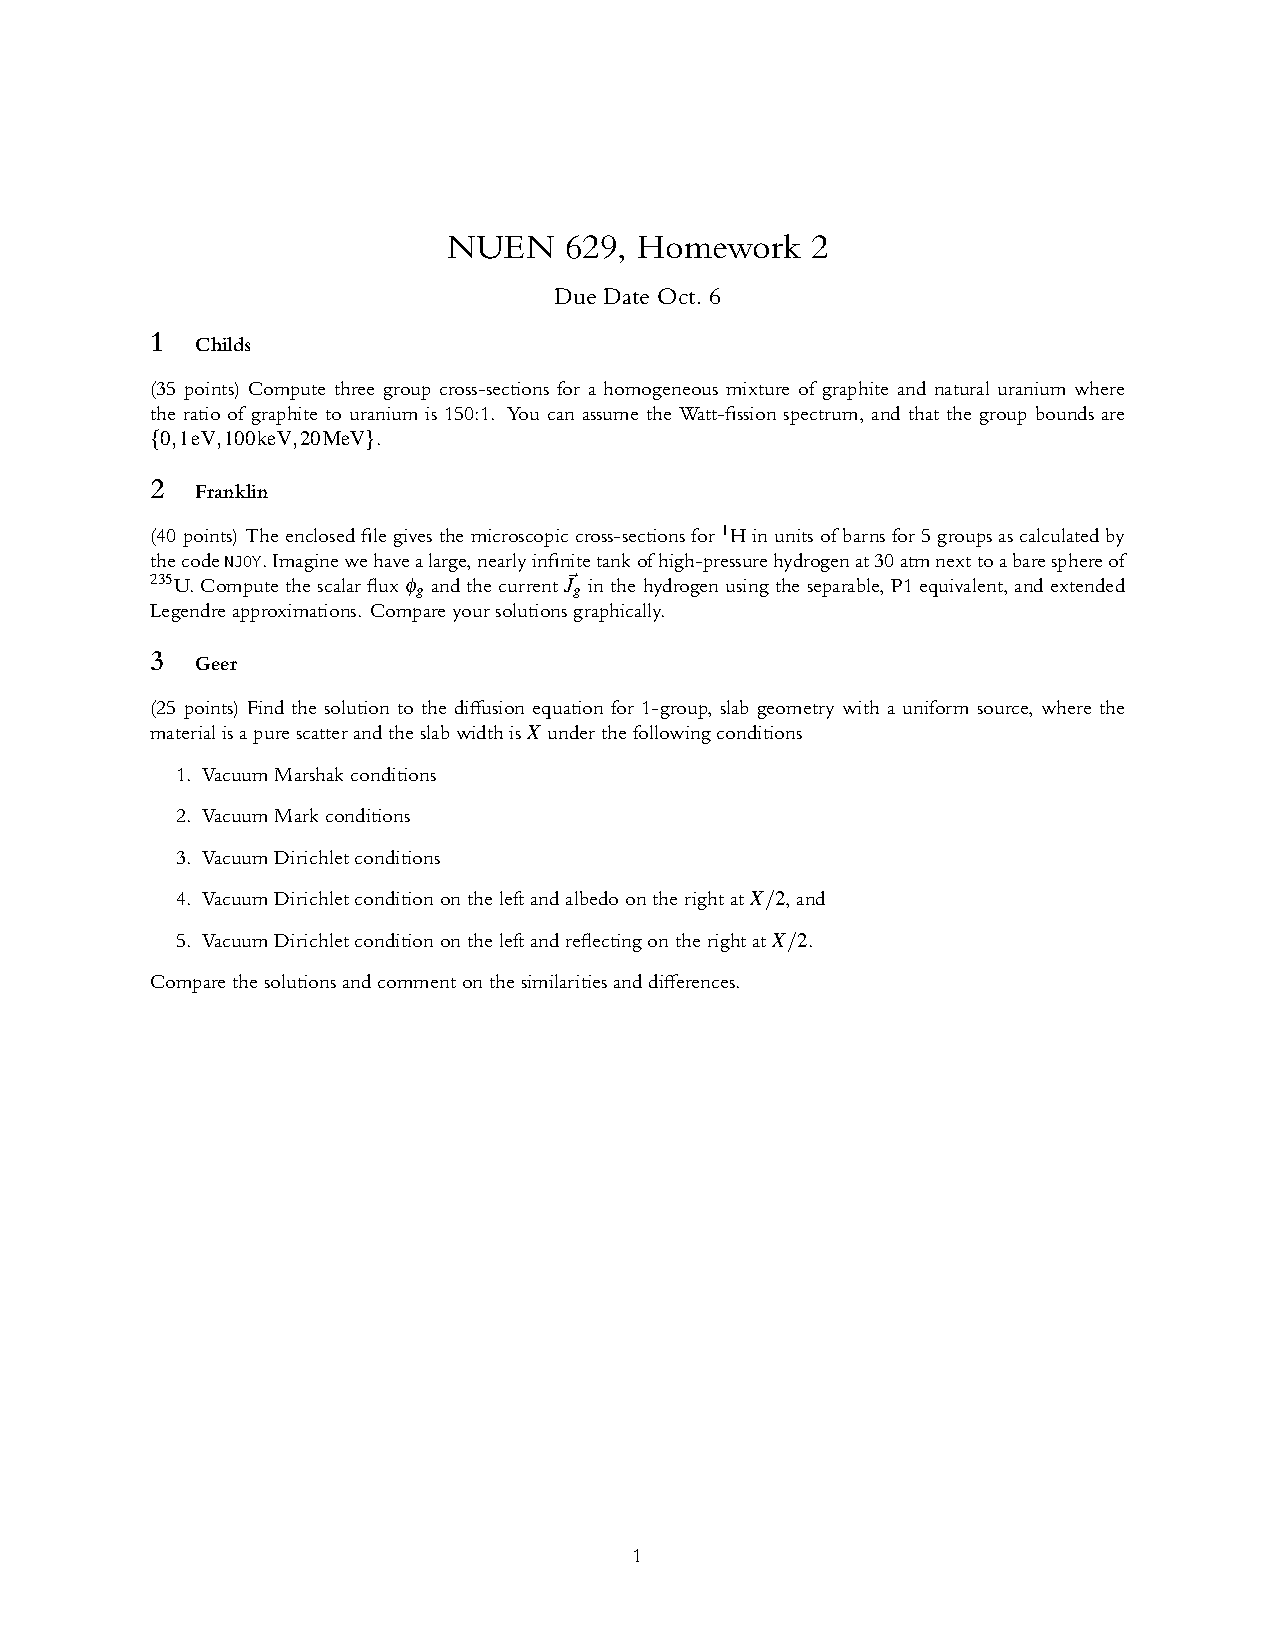
\includepdf{Homework2.pdf}

\begin{solnum}{1}
    
Several approximations were made to simplify the process.  First, graphite is
approximated as elemental Carbon, with molar mass 12.0107 (g/mol).  This was done because there is not a human
friendly form of the graphite cross sections available on NNDC and elemental Carbon
will have similar scattering properties, except for at low energies where diffraction is
possible.  A plot of the elastic and total cross sections for elemental Carbon from
NNDC are given below.
\begin{figure}[h!]
\centering
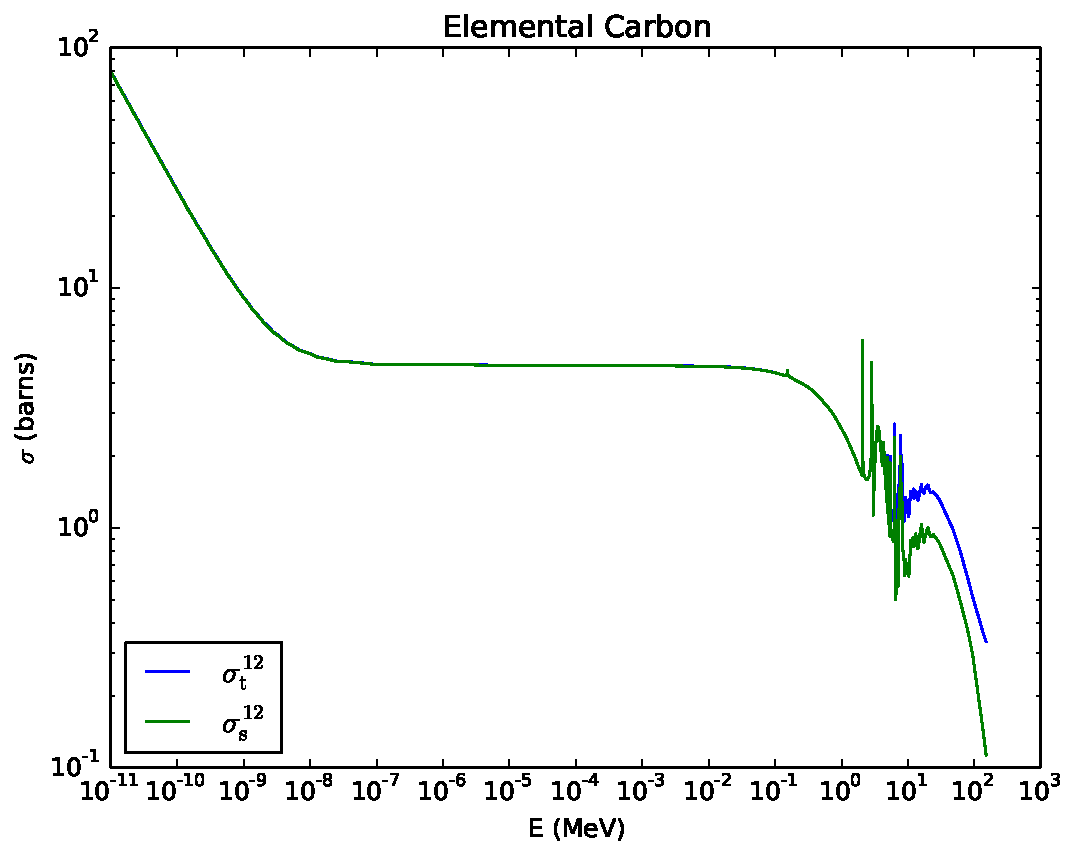
\includegraphics[width=0.5\textwidth]{carb_cx.pdf}
\end{figure}



The ratio of 150:1 for graphite to natural uranium is assumed to be an of
atomic ratio.  Natural uranium is
taken to be 0.72\% $^{235}$U and the remainder $^{238}$U, by atom percentage. 
The total cross section
is assumed to only consist of elastic scattering, fission, and removal events.

We follow a similar procedure to the one in lab.  For an infinite medium, with
fine-group cross sections, the balance equation becomes
\begin{multline}
    N^{U}\sum_{j} \gamma_j \sigma_t^j(E) \psi(\mu,E) = N^{U}\sum_{j} \gamma_j
    \frac{1}{2} \int\limits_0^\infty \d E' \sigma_s^j (E'\ra E)\phi(E') + \\
    N^U\frac{\chi(E)}{2k} \int_0^\infty\d E' \left(\gamma_{238}\nubar\sigma_f^{238} +
    \gamma_{235}\nubar\sigma_f^{235}\right)\phi(E'),
\end{multline}
where $j$ indicates the $j$-th isotope, $N^U$ is the atom density of natural uranium
in the system, and $\gamma_j$ is 150, 0.9928, and 0.0072 for Carbon, \iso{U}{238},
and \iso{U}{235}, respectively.  It is assumed $\chi(E)$ is the same for \iso{U}{238}
and \iso{U}{235}, given by the Watt spectrum from class
\begin{equation}
    \chi(E) = 0.4865 \sinh(\sqrt{2E})e^{-E}.
\end{equation}
We now simplify by normalizing such that the energy integrated fission source has a
magnitude of 1.  We also assume all scattering events result in the average
scattering energy loss, which, assuming isotropic scattering in the center of mass
frame, gives an average outgoing energy of 
\begin{equation}
    \langle E\rangle = \frac{A^2 + 1}{(A+1)^2}E'
\end{equation}
in the lab frame.  With this simplificiation, only a particular $E'$ governed by the above equation can scatter
into $E$, so the the elastic scattering source for the $j$-th term in the summation can be simplified as
\begin{align}
    \int_0^\infty \d E' \sigma_s^j(E')P(E'\ra E)\phi(E') &= \int_0^\infty \d
    E'\sigma_s^j(E')\delta\left(E' - E \frac{E'}{\langle E \rangle}\right) \phi(E') \\
    &= \sigma_s^j\left(\frac{(A+1)^2}{A^2+1}E\right) \phi\left(\frac{(A+1)^2}{A^2+1}E\right) \\
\end{align}
where $A$ is the atomic mass number for the $j$-th isotope, approximated as 12.0107 for elemental carbon.
Substituting back into the original equation and integrating over angle gives the
final equation for the scalar flux as
\begin{equation}
    \sum_{j} \gamma_j \sigma_t^j(E) \phi(E) = \sum_{j} \gamma_j \sigma_s^j \left(\frac{(A+1)^2}{A^2+1}E\right) \phi\left(\frac{(A+1)^2}{A^2+1}E\right) 
   + {\chi(E)} .
\end{equation}
We solve this equation with the Jacobi iteration
\begin{equation}
    \sum_{j} \gamma_j \sigma_t^j(E) \phi^{(k)}(E) = \sum_{j} \gamma_j \sigma_s^j
    \left(\frac{(A+1)^2}{A^2+1}E\right) \phi^{(k-1)}\left(\frac{(A+1)^2}{A^2+1}E\right) 
   + {\chi(E)} .
\end{equation}
with an initial guess of $\phi^{(0)}(E)=0$.
To approximate the continuous energy cross sections and $\phi(E)$ we simply evaluate the
above iteration at each of the energy points of the fine group cross sections. The
points are defined using the union of the total cross section energy grids of all
isotopes.  A linear interpolation (python interp1D default interpolation) is used between energy points when one
cross section is coarser than others. For evaluation above the maximum energy for a
given cross section, the value of the cross section at the maximum energy is used.




\end{solnum}

%\includepdf[pages={1}]{p1p3.pdf}
\clearpage
    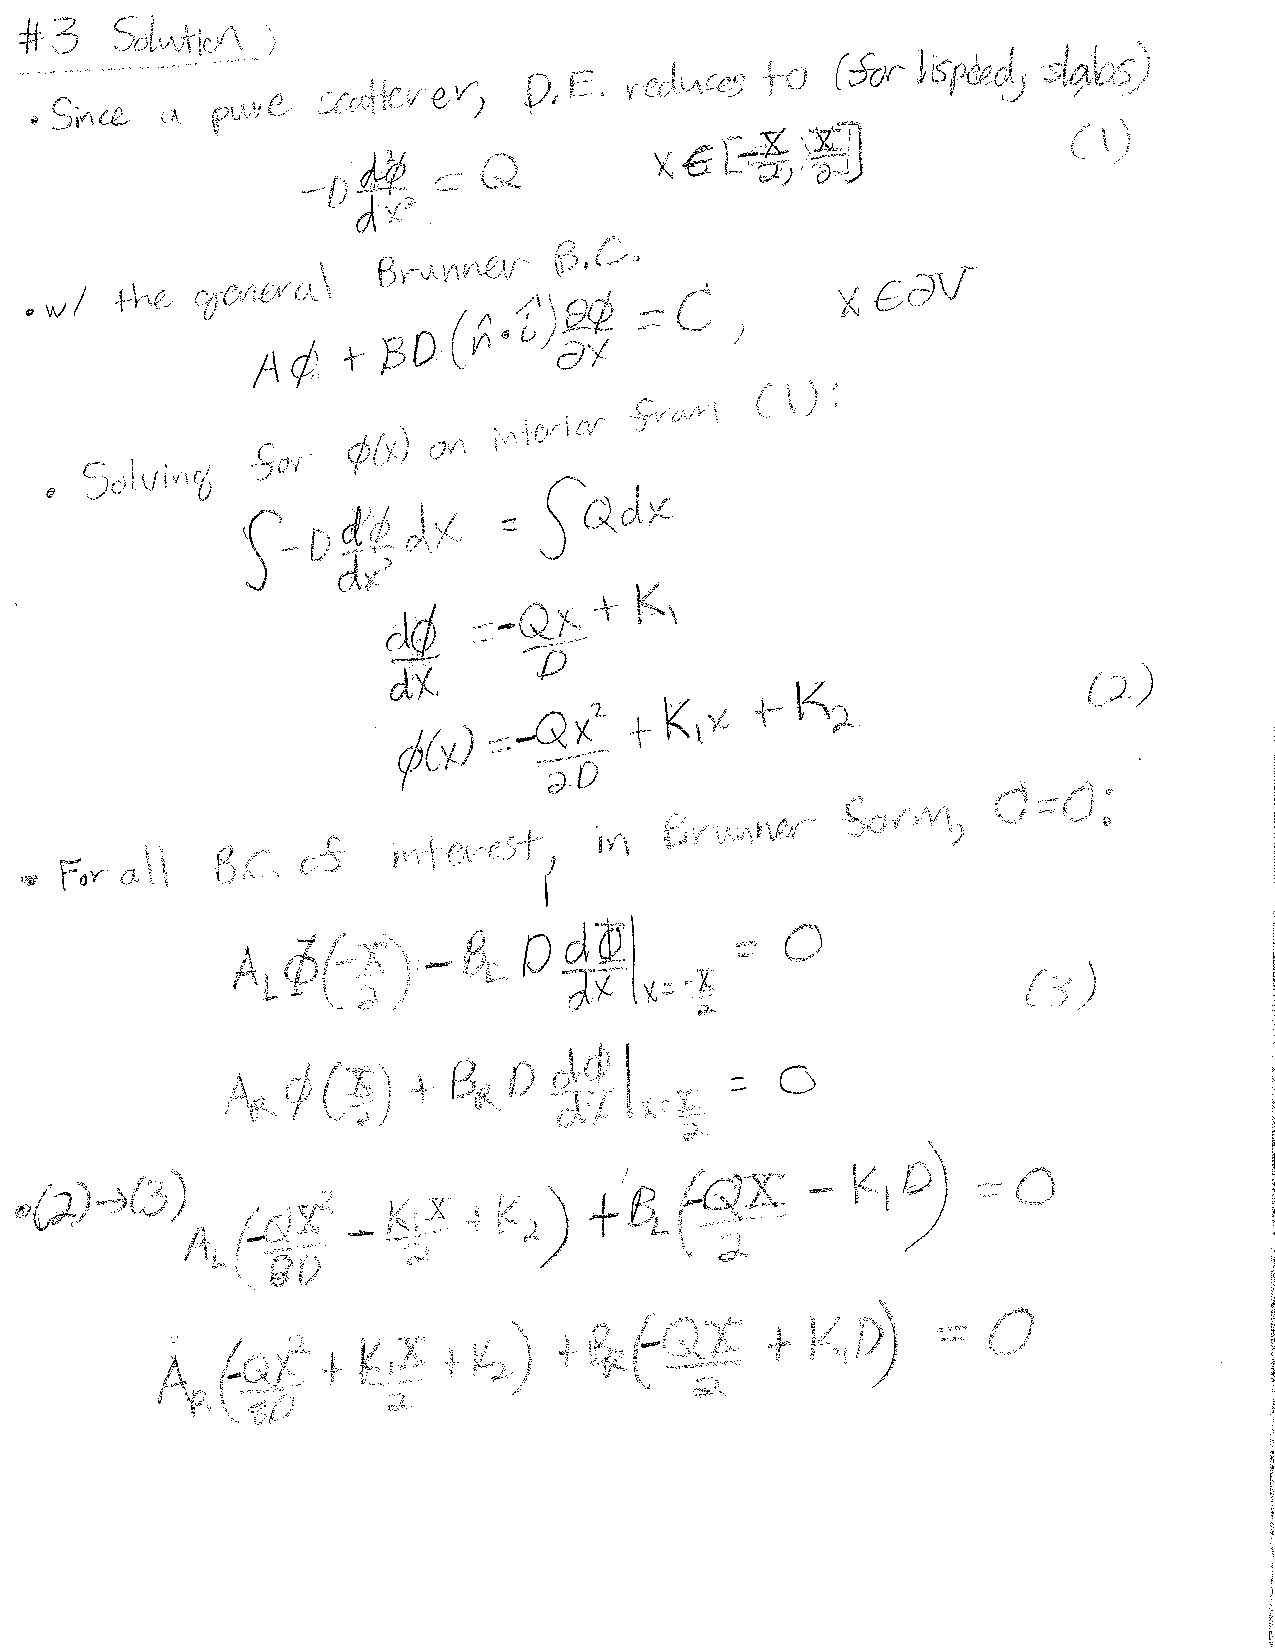
\includepdf[pages={1-2}]{p3.pdf}
    A summary of the solutions obtained for each of the boundary conditions is given
    in the table below.  Each solution was checked to ensure they satisfy the
    boundary conditions.
    \begin{table}[h]
        \centering
        \caption{Solutions with different boundary conditions for  a pure scatter for slab of width $X$ centered at
        $x=0$.}
        \begin{tabular}{|c|c|c|} \hline
            Left BC & Right BC & $\phi(x)$ \\ \hline
            Vacuum Marshak & Vacuum Marshak & $\phi(x) = Q\left(\frac{X^2}{8D} + X-\frac{x^2}{2D} 
            \right)            $ \\ 
            Vacuum Mark & Vacuum Marshak & $\phi(x) = Q\left(
            \frac{X^2}{8D} + \frac{X\sqrt{3}}{2}-\frac{x^2}{2D}\right)$ \\ 
            Vacuum Dirichlet  & Vacuum Dirichlet & $\phi(x) = \frac{Q}{2D}\left( 
            \frac{X^2}{4} - x^2\right)  $ \\ 
            Vacuum Dirichlet    & Albedo  & $\phi(x) = -\frac{Qx^2}{2D} +
            QxX\left(\frac{1+\A\frac{X}{2D}}{\A X + D} - \frac{1}{2D}  \right) +
            Q\frac{X^2}{2} \left(\frac{1+\A\frac{X}{2D}}{\A X +
            D}-\frac{1}{4D}\right) $ \\
            Vacuum Dirichlet    & Reflecting & $\phi(x) =
            \frac{Q}{2D}\left(\frac{3X^2}{4} + xX  - {x^2}\right)$ \\ \hline
        \end{tabular}
    \end{table}
\clearpage


\end{document}

